\documentclass[a4paper,12pt]{article}
%%%%%%%%%%%%%%%%%%%%%%%%%%%%%%%%%%%%%%%%%%%%%%%%%%%%%%%%%%%%%%%%%%%%%%%%%%%%%%%%%%%%%%%%%%%%%%%%%%%%%%%%%%%%%%%%%%%%%%%%%%%%%%%%%%%%%%%%%%%%%%%%%%%%%%%%%%%%%%%%%%%%%%%%%%%%%%%%%%%%%%%%%%%%%%%%%%%%%%%%%%%%%%%%%%%%%%%%%%%%%%%%%%%%%%%%%%%%%%%%%%%%%%%%%%%%
\usepackage{eurosym}
\usepackage{vmargin}
\usepackage{amsmath}
\usepackage{graphics}
\usepackage{epsfig}
\usepackage{framed}
\usepackage{subfigure}
\usepackage{fancyhdr}

\setcounter{MaxMatrixCols}{10}
%TCIDATA{OutputFilter=LATEX.DLL}
%TCIDATA{Version=5.00.0.2570}
%TCIDATA{<META NAME="SaveForMode"CONTENT="1">}
%TCIDATA{LastRevised=Wednesday, February 23, 201113:24:34}
%TCIDATA{<META NAME="GraphicsSave" CONTENT="32">}
%TCIDATA{Language=American English}

\pagestyle{fancy}
\setmarginsrb{20mm}{0mm}{20mm}{25mm}{12mm}{11mm}{0mm}{11mm}
\lhead{MA4128} \rhead{Kevin O'Brien} \chead{Week 8 Part B} %\input{tcilatex}

%http://www.electronics.dit.ie/staff/ysemenova/Opto2/CO_IntroLab.pdf
\begin{document}


\subsection{Akaike Information Criterion}


Akaike's information criterionis a measure of the goodness of fit of
an estimated statistical model. The AIC was developed by Hirotsugu Akaike under the name of ``an information criterion" in 1971. The AIC is a \textbf{\textit{model selection}} tool i.e. a method of comparing two
or more candidate regression models. The AIC methodology attempts to find the model that best explains the data with a minimum of parameters. (i.e. in keeping with the law of parsimony)

The AIC is calculated using the "likelihood function" and the number of parameters ( Likelihood function : not on course). The likelihood value is generally given in code output, as a complement to the AIC.
Given a data set, several competing models may be ranked according to their AIC, with the one having the lowest AIC being the best. (Although, a difference in AIC values of less than two is considered negligible).

The Akaike information criterion is a measure of the relative goodness of fit of a statistical model. It was developed by Hirotsugu Akaike, under the name of "an information criterion" (AIC), and was first published by Akaike in 1974.
\bigskip
%AIC provides a means for comparison among models—a tool for model selection.
%\bigskip
%AIC is good for prediction.\\

\[\mbox{AIC} = 2p - 2\ln(L)\]

\begin{itemize}
	\item $p$ is the number of free model parameters.
	\item $L$ is the value of the Likelihood function for the model in question.
	\item For AIC to be optimal, $n$ must be large compared to $p$.\\
\end{itemize}
\subsubsection{Schwarz's Bayesian Information Criterion}
An alternative to the AIC is the Schwarz BIC, which additionally takes into account the sample size $n$.

\[\mbox{BIC} = p\ln{n} - 2\ln(L)\]



\section{Information Criterions}


We define two types of information criterion: the Bayesian Information
Criterion (BIC) and the Akaike Information Criterion (AIC). In AIC and BIC, we choose the model that
has the minimum value of:
\[AIC = −2log(L)+2m,\]
\[BIC = −2log(L)+mlogn\]

where
\begin{itemize}
\item L is the likelihood of the data with a certain model,
\item n is the number of observations and
\item m is the number of parameters in the model.
\end{itemize}
\subsection{AIC}
The Akaike information criterion is a measure of the relative \textbf{goodness of fit} of a statistical model.

When using the AIC for selecting the parametric model class, choose
the model for which the AIC value is lowest.


\subsection{Akaike Information Criterion}


Akaike's information criterionis a measure of the goodness of fit of
an estimated statistical model. The AIC was developed by Hirotsugu Akaike under the name of ``an information criterion" in 1971. The AIC is a \textbf{\textit{model selection}} tool i.e. a method of comparing two
or more candidate regression models. The AIC methodology attempts to find the model that best explains the data with a minimum of parameters. (i.e. in keeping with the law of parsimony)

The AIC is calculated using the "likelihood function" and the number of parameters ( Likelihood function : not on course). The likelihood value is generally given in code output, as a complement to the AIC.
Given a data set, several competing models may be ranked according to their AIC, with the one having the lowest AIC being the best. (Although, a difference in AIC values of less than two is considered negligible).

The Akaike information criterion is a measure of the relative goodness of fit of a statistical model. It was developed by Hirotsugu Akaike, under the name of "an information criterion" (AIC), and was first published by Akaike in 1974.
\bigskip
%AIC provides a means for comparison among models—a tool for model selection.
%\bigskip
%AIC is good for prediction.\\

\[\mbox{AIC} = 2p - 2\ln(L)\]

\begin{itemize}
\item $p$ is the number of free model parameters.
\item $L$ is the value of the Likelihood function for the model in question.
\item For AIC to be optimal, $n$ must be large compared to $p$.\\
\end{itemize}
\subsubsection{Schwarz's Bayesian Information Criterion}
An alternative to the AIC is the Schwarz BIC, which additionally takes into account the sample size $n$.

\[\mbox{BIC} = p\ln{n} - 2\ln(L)\]


\subsection{AIC and BIC in Two-Step Cluster Analysis}

(Removed from Last Week's Class due to Version Update)

Two-Step Cluster Analysis guides the decision of how many clusters to retain from the data by
calculating measures-of-fit such as \textbf{\textit{Akaike’s Information Criterion (AIC)}} or \textbf{\textit{Bayes Information Criterion (BIC)}}.

These are relative measures of goodness-of-fit and are used to compare different
solutions with different numbers of segments.(``Relative" means that these criteria
are not scaled on a range of, for example, 0 to 1 but can generally take any value.)


\textbf{\textit{Important}}: Compared to an alternative solution with a different number of segments, smaller
values in AIC or BIC indicate an increased fit.

SPSS computes solutions for different segment numbers (up to the maximum number of segments specified before) and
chooses the appropriate solution by looking for the smallest value in the chosen
criterion. However, which criterion should we choose?
\begin{itemize}
\item AIC is well-known for
overestimating the correct number of segments
\item BIC has a slight tendency
to underestimate this number.
\end{itemize}

Thus, it is worthwhile comparing the clustering
outcomes of both criteria and selecting a smaller number of segments than
actually indicated by AIC. Nevertheless, when running two separate analyses,
one based on AIC and the other based on BIC, SPSS usually renders the same
results.

Once you make some choices or do nothing and go with the defaults, the clusters are
formed. At this point, you can consider whether the number of clusters is ``good". If
automated cluster selection is used, SPSS prints a table of statistics for different
numbers of clusters, an excerpt of which is shown in the figure below. You are interested
in finding the number of clusters at which the Schwarz BIC becomes small , but also the change in BIC between
adjacent number of clusters is small. 

The decision of how much benefit accrued by another cluster is very subjective. In addition to the BIC, a high ratio of distance of measures is desirable. In the figure below, the number of clusters with this highest ratio is three.

\begin{figure}[h!]
\begin{centering}
  % Requires \usepackage{graphicx}
  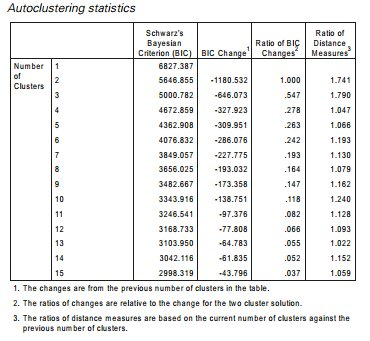
\includegraphics[width=10cm]{TwoStep1.jpg}\\
  \caption{Schwarz Bayesian Information Criterion}
\end{centering}
\end{figure}


Information Criterions
We define two types of information criterion: the Akaike Information Criterion (AIC) and the
Schwarz’s Bayesian Information Criterion (BIC). The Akaike information criterion is a measure
of the relative goodness of fit of a statistical model.
AIC = 2p − 2 ln(L)


%=================================================%
\begin{itemize}
\item p is the number of predictor variables in the model.
\item L is the value of the Likelihood function for the model in question.
\item For AIC to be optimal, n must be large compared to p.
\end{itemize}

An alternative to the AIC is the Schwarz BIC, which additionally takes into account the
sample size n.
BIC = p ln n − 2 ln(L)
When using the AIC (or BIC) for selecting the optimal model, we choose the model for which
the AIC (or BIC) value is lowest.


Akaike Information Criterion

\begin{itemize}
\item Akaike’s information criterionis a measure of the goodness of fit of an estimated statistical
model. The AIC was developed by Hirotsugu Akaike under the name of “an information
criterion” in 1971.
\item The AIC is a model selection tool i.e. a method of comparing two or more candidate
regression models. The AIC methodology attempts to find the model that best explains
the data with a minimum of parameters. (i.e. in keeping with the law of parsimony)
\item The AIC is calculated using the ”likelihood function” and the number of parameters .
The likelihood value is generally given in code output, as a complement to the AIC.
(Likelihood function is not on our course)
\item Given a data set, several competing models may be ranked according to their AIC, with
the one having the lowest AIC being the best. (Although, a difference in AIC values of
less than two is considered negligible).

\end{itemize}

%=================================================%
\subsection{Model Metrics for Logistic Regression Models}
\begin{itemize}
\item In order to understand how much variation in the dependent variable can be explained
by a logistic regression model (the equivalent of R 2 in multiple regression), you should
consult Model Summary statistics.
\item Although there is no close analogous statistic in logistic regression to the coefficient of
determination R 2 the Model Summary Table provides some approximations.
\item Logistic regression does not have an equivalent to the R-squared that is found in OLS
regression; however, many researchers have tried to come up with one.
\item The SPSS output table below contains the Cox \& Snell R Square and Nagelkerke R Square
values, which are both methods of calculating the explained variation. These values are
sometimes referred to as pseudo R 2 values (and will have lower values than in multiple
regression).
\item However, they are interpreted in the same manner, but with more caution. Therefore,
the explained variation in the dependent variable based on our model ranges from 24.0%
to 33.0\%, depending on whether you reference the Cox \& Snell R 2 or Nagelkerke R 2
methods, respectively.
\item Nagelkerke R 2 is a modification of Cox \& Snell R 2 , the latter of which cannot achieve a
value of 1. For this reason, it is preferable to report the Nagelkerke R 2 value.
\item The Nagelkerke modification that does range from 0 to 1 is a more reliable measure of
the relationship.
\item Nagelkerkes R 2 will normally be higher than the Cox and Snell measure.
Figure 1: SPSS output
\item Cox and Snells R-Square attempts to imitate multiple R-Square based on likelihood, but
its maximum can be (and usually is) less than 1.0, making it difficult to interpret. Here
it is indicating that 55.2% of the variation in the dependent variable is explained by the
logistic model.
\end{itemize}

%=================================================%
\subsection{Pseudo R-squares}
\begin{itemize}
\item Cox \& Snell R Square and Nagelkerke R Square are two measures from the pseudo
R-squares family of measures.
\item There are a wide variety of pseudo-R-square statistics (these are only two of them).
Because this statistic does not mean what R-squared means in OLS regression (the pro-
portion of variance explained by the predictors), we suggest interpreting this statistic with
great caution.
\end{itemize}
%=================================================%
\subsection{Cox \& Snell R Square}
Cox and Snell’s R-Square is an attempt to imitate the interpretation of multiple R-Square based
on the likelihood, but its maximum can be (and usually is) less than 1.0, making it difficult to
interpret. It is part of SPSS output.
%=================================================%
\subsection{Nagelkerke’s R-Square}
\begin{itemize}
\item Nagelkerkes R 2 is part of SPSS output in the Model Summary table and is the most-
reported of the R-squared estimates.
\item In our case it is 0.737, indicating a moderately strong relationship of 73.7% between the
predictors and the prediction.
\item Nagelkerke’s R-Square is a further modification of the Cox and Snell coefficient to assure
that it can vary from 0 to 1. Nagelkerke’s R-Square will normally be higher than the Cox
and Snell measure. It is part of SPSS output and is the most-reported of the R-squared
estimates.
\end{itemize}
\end{document}
